\documentclass[12pt]{article}
\usepackage[letterpaper, left=0.6in, right=0.6in, top=0.95in, bottom=0.95in,
  headheight=15pt, headsep=0.25in, footskip=0.45in]{geometry}
\usepackage[T1]{fontenc}
\usepackage[default]{sourcesanspro}
\usepackage{inconsolata}
\usepackage{textcomp}
\usepackage{microtype}
\usepackage{tikz}
\usetikzlibrary{arrows.meta}
\usepackage{fancyhdr}
\pagestyle{fancy}
\fancyhf{}
\fancyhead[L]{Week 4 / Stars and wheels / Grades 2--3}
\fancyfoot[L]{Bellingham Math Circle / Week 4 / F04-M-v4}
\fancyfoot[R]{\thepage}
\renewcommand{\headrulewidth}{0pt}
\setlength{\parindent}{0pt}
\setlength{\parskip}{0pt}
\newcommand{\prob}[1]{\textbf{Problem #1:}}
\newcommand{\bx}{\hspace{0.07in}\begingroup\setlength{\fboxsep}{0pt}\setlength{\fboxrule}{0.8pt}\raisebox{-0.11in}{\framebox[0.42in]{\rule{0pt}{0.34in}}}\endgroup}
\newcommand{\blank}{\rule[-3pt]{0.85in}{0.6pt}}
\pagenumbering{arabic}
\begin{document}
\par\vspace{0in}\noindent To draw hop 3 on a ring of dots, start at any dot and draw a straight line to the dot 3 places clockwise. Keep hopping 3 until you are back where you started. If some dots still have no line, start again at one of them, and stop when every dot has a line.\par
\par\vspace{0.16in}\noindent \prob{1} Draw hop 1, hop 2, hop 3 and hop 4 on these rings of 8 dots. Write how many times you started in the box under each drawing.\par
\par\vspace{0.3in}\noindent\makebox[\textwidth][s]{\hfill \begin{tikzpicture}[x=1in,y=1in]
\useasboundingbox (-1.8,-1.9) rectangle (1.8,1.4);
\draw[black!25, line width=0.5pt] (0,0) circle (1.3);
\fill[black] (0,1.3) circle (0.045);
\fill[black] (0.9192,0.9192) circle (0.045);
\fill[black] (1.3,0) circle (0.045);
\fill[black] (0.9192,-0.9192) circle (0.045);
\fill[black] (0,-1.3) circle (0.045);
\fill[black] (-0.9192,-0.9192) circle (0.045);
\fill[black] (-1.3,0) circle (0.045);
\fill[black] (-0.9192,0.9192) circle (0.045);
\node[font=\normalsize] at (0,-1.6) {hop 1\qquad\bx};
\end{tikzpicture}\hfill \begin{tikzpicture}[x=1in,y=1in]
\useasboundingbox (-1.8,-1.9) rectangle (1.8,1.4);
\draw[black!25, line width=0.5pt] (0,0) circle (1.3);
\fill[black] (0,1.3) circle (0.045);
\fill[black] (0.9192,0.9192) circle (0.045);
\fill[black] (1.3,0) circle (0.045);
\fill[black] (0.9192,-0.9192) circle (0.045);
\fill[black] (0,-1.3) circle (0.045);
\fill[black] (-0.9192,-0.9192) circle (0.045);
\fill[black] (-1.3,0) circle (0.045);
\fill[black] (-0.9192,0.9192) circle (0.045);
\node[font=\normalsize] at (0,-1.6) {hop 2\qquad\bx};
\end{tikzpicture}\hfill}\par
\par\vspace{0.4in}\noindent\makebox[\textwidth][s]{\hfill \begin{tikzpicture}[x=1in,y=1in]
\useasboundingbox (-1.8,-1.9) rectangle (1.8,1.4);
\draw[black!25, line width=0.5pt] (0,0) circle (1.3);
\fill[black] (0,1.3) circle (0.045);
\fill[black] (0.9192,0.9192) circle (0.045);
\fill[black] (1.3,0) circle (0.045);
\fill[black] (0.9192,-0.9192) circle (0.045);
\fill[black] (0,-1.3) circle (0.045);
\fill[black] (-0.9192,-0.9192) circle (0.045);
\fill[black] (-1.3,0) circle (0.045);
\fill[black] (-0.9192,0.9192) circle (0.045);
\node[font=\normalsize] at (0,-1.6) {hop 3\qquad\bx};
\end{tikzpicture}\hfill \begin{tikzpicture}[x=1in,y=1in]
\useasboundingbox (-1.8,-1.9) rectangle (1.8,1.4);
\draw[black!25, line width=0.5pt] (0,0) circle (1.3);
\fill[black] (0,1.3) circle (0.045);
\fill[black] (0.9192,0.9192) circle (0.045);
\fill[black] (1.3,0) circle (0.045);
\fill[black] (0.9192,-0.9192) circle (0.045);
\fill[black] (0,-1.3) circle (0.045);
\fill[black] (-0.9192,-0.9192) circle (0.045);
\fill[black] (-1.3,0) circle (0.045);
\fill[black] (-0.9192,0.9192) circle (0.045);
\node[font=\normalsize] at (0,-1.6) {hop 4\qquad\bx};
\end{tikzpicture}\hfill}\par
\vfill

\newpage
\par\vspace{0in}\noindent \prob{2} Draw hop 2, hop 3, hop 4 and hop 5 on these rings of 10 dots. Write how many times you started in the box under each drawing.\par
\par\vspace{0.35in}\noindent\makebox[\textwidth][s]{\hfill \begin{tikzpicture}[x=1in,y=1in]
\useasboundingbox (-1.8,-1.9) rectangle (1.8,1.4);
\draw[black!25, line width=0.5pt] (0,0) circle (1.3);
\fill[black] (0,1.3) circle (0.045);
\fill[black] (0.7641,1.0517) circle (0.045);
\fill[black] (1.2364,0.4017) circle (0.045);
\fill[black] (1.2364,-0.4017) circle (0.045);
\fill[black] (0.7641,-1.0517) circle (0.045);
\fill[black] (0,-1.3) circle (0.045);
\fill[black] (-0.7641,-1.0517) circle (0.045);
\fill[black] (-1.2364,-0.4017) circle (0.045);
\fill[black] (-1.2364,0.4017) circle (0.045);
\fill[black] (-0.7641,1.0517) circle (0.045);
\node[font=\normalsize] at (0,-1.6) {hop 2\qquad\bx};
\end{tikzpicture}\hfill \begin{tikzpicture}[x=1in,y=1in]
\useasboundingbox (-1.8,-1.9) rectangle (1.8,1.4);
\draw[black!25, line width=0.5pt] (0,0) circle (1.3);
\fill[black] (0,1.3) circle (0.045);
\fill[black] (0.7641,1.0517) circle (0.045);
\fill[black] (1.2364,0.4017) circle (0.045);
\fill[black] (1.2364,-0.4017) circle (0.045);
\fill[black] (0.7641,-1.0517) circle (0.045);
\fill[black] (0,-1.3) circle (0.045);
\fill[black] (-0.7641,-1.0517) circle (0.045);
\fill[black] (-1.2364,-0.4017) circle (0.045);
\fill[black] (-1.2364,0.4017) circle (0.045);
\fill[black] (-0.7641,1.0517) circle (0.045);
\node[font=\normalsize] at (0,-1.6) {hop 3\qquad\bx};
\end{tikzpicture}\hfill}\par
\par\vspace{0.45in}\noindent\makebox[\textwidth][s]{\hfill \begin{tikzpicture}[x=1in,y=1in]
\useasboundingbox (-1.8,-1.9) rectangle (1.8,1.4);
\draw[black!25, line width=0.5pt] (0,0) circle (1.3);
\fill[black] (0,1.3) circle (0.045);
\fill[black] (0.7641,1.0517) circle (0.045);
\fill[black] (1.2364,0.4017) circle (0.045);
\fill[black] (1.2364,-0.4017) circle (0.045);
\fill[black] (0.7641,-1.0517) circle (0.045);
\fill[black] (0,-1.3) circle (0.045);
\fill[black] (-0.7641,-1.0517) circle (0.045);
\fill[black] (-1.2364,-0.4017) circle (0.045);
\fill[black] (-1.2364,0.4017) circle (0.045);
\fill[black] (-0.7641,1.0517) circle (0.045);
\node[font=\normalsize] at (0,-1.6) {hop 4\qquad\bx};
\end{tikzpicture}\hfill \begin{tikzpicture}[x=1in,y=1in]
\useasboundingbox (-1.8,-1.9) rectangle (1.8,1.4);
\draw[black!25, line width=0.5pt] (0,0) circle (1.3);
\fill[black] (0,1.3) circle (0.045);
\fill[black] (0.7641,1.0517) circle (0.045);
\fill[black] (1.2364,0.4017) circle (0.045);
\fill[black] (1.2364,-0.4017) circle (0.045);
\fill[black] (0.7641,-1.0517) circle (0.045);
\fill[black] (0,-1.3) circle (0.045);
\fill[black] (-0.7641,-1.0517) circle (0.045);
\fill[black] (-1.2364,-0.4017) circle (0.045);
\fill[black] (-1.2364,0.4017) circle (0.045);
\fill[black] (-0.7641,1.0517) circle (0.045);
\node[font=\normalsize] at (0,-1.6) {hop 5\qquad\bx};
\end{tikzpicture}\hfill}\par
\vfill

\newpage
\par\vspace{0in}\noindent \prob{3} Before you draw each hop on these rings of 12 dots, guess how many times you will start and write your guess. Then draw it and write how many times you did start.\par
\par\vspace{0.3in}\noindent\makebox[\textwidth][s]{\hfill 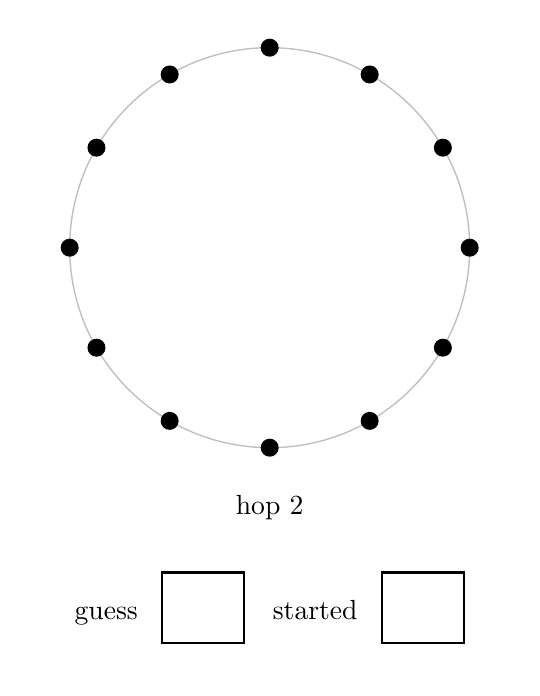
\begin{tikzpicture}[x=1in,y=1in]
\useasboundingbox (-1.21,-2.1) rectangle (1.21,1.1);
\draw[black!25, line width=0.5pt] (0,0) circle (1);
\fill[black] (0,1) circle (0.045);
\fill[black] (0.5,0.866) circle (0.045);
\fill[black] (0.866,0.5) circle (0.045);
\fill[black] (1,0) circle (0.045);
\fill[black] (0.866,-0.5) circle (0.045);
\fill[black] (0.5,-0.866) circle (0.045);
\fill[black] (0,-1) circle (0.045);
\fill[black] (-0.5,-0.866) circle (0.045);
\fill[black] (-0.866,-0.5) circle (0.045);
\fill[black] (-1,0) circle (0.045);
\fill[black] (-0.866,0.5) circle (0.045);
\fill[black] (-0.5,0.866) circle (0.045);
\node[font=\normalsize] at (0,-1.3) {hop 2};
\node[font=\normalsize] at (0,-1.8) {guess~\bx\quad started~\bx};
\end{tikzpicture}\hfill 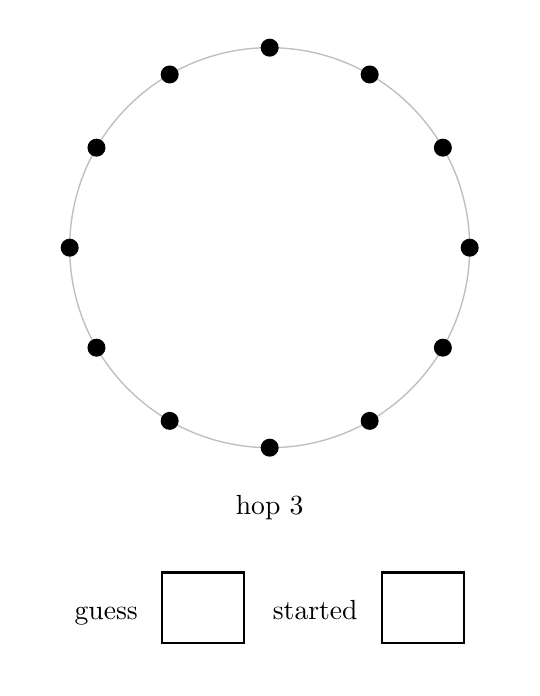
\begin{tikzpicture}[x=1in,y=1in]
\useasboundingbox (-1.21,-2.1) rectangle (1.21,1.1);
\draw[black!25, line width=0.5pt] (0,0) circle (1);
\fill[black] (0,1) circle (0.045);
\fill[black] (0.5,0.866) circle (0.045);
\fill[black] (0.866,0.5) circle (0.045);
\fill[black] (1,0) circle (0.045);
\fill[black] (0.866,-0.5) circle (0.045);
\fill[black] (0.5,-0.866) circle (0.045);
\fill[black] (0,-1) circle (0.045);
\fill[black] (-0.5,-0.866) circle (0.045);
\fill[black] (-0.866,-0.5) circle (0.045);
\fill[black] (-1,0) circle (0.045);
\fill[black] (-0.866,0.5) circle (0.045);
\fill[black] (-0.5,0.866) circle (0.045);
\node[font=\normalsize] at (0,-1.3) {hop 3};
\node[font=\normalsize] at (0,-1.8) {guess~\bx\quad started~\bx};
\end{tikzpicture}\hfill 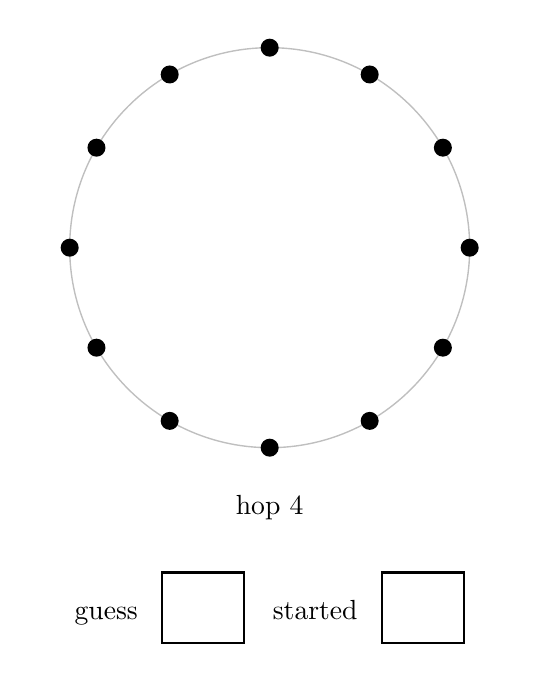
\begin{tikzpicture}[x=1in,y=1in]
\useasboundingbox (-1.21,-2.1) rectangle (1.21,1.1);
\draw[black!25, line width=0.5pt] (0,0) circle (1);
\fill[black] (0,1) circle (0.045);
\fill[black] (0.5,0.866) circle (0.045);
\fill[black] (0.866,0.5) circle (0.045);
\fill[black] (1,0) circle (0.045);
\fill[black] (0.866,-0.5) circle (0.045);
\fill[black] (0.5,-0.866) circle (0.045);
\fill[black] (0,-1) circle (0.045);
\fill[black] (-0.5,-0.866) circle (0.045);
\fill[black] (-0.866,-0.5) circle (0.045);
\fill[black] (-1,0) circle (0.045);
\fill[black] (-0.866,0.5) circle (0.045);
\fill[black] (-0.5,0.866) circle (0.045);
\node[font=\normalsize] at (0,-1.3) {hop 4};
\node[font=\normalsize] at (0,-1.8) {guess~\bx\quad started~\bx};
\end{tikzpicture}\hfill}\par
\par\vspace{0.45in}\noindent\makebox[\textwidth][s]{\hfill 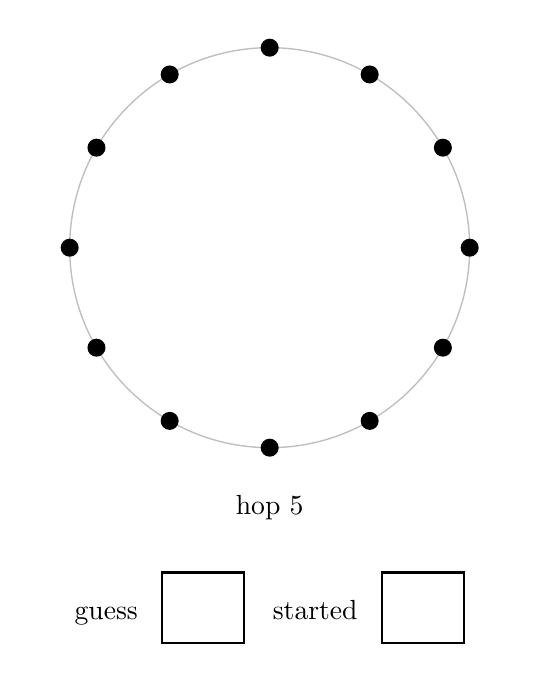
\begin{tikzpicture}[x=1in,y=1in]
\useasboundingbox (-1.21,-2.1) rectangle (1.21,1.1);
\draw[black!25, line width=0.5pt] (0,0) circle (1);
\fill[black] (0,1) circle (0.045);
\fill[black] (0.5,0.866) circle (0.045);
\fill[black] (0.866,0.5) circle (0.045);
\fill[black] (1,0) circle (0.045);
\fill[black] (0.866,-0.5) circle (0.045);
\fill[black] (0.5,-0.866) circle (0.045);
\fill[black] (0,-1) circle (0.045);
\fill[black] (-0.5,-0.866) circle (0.045);
\fill[black] (-0.866,-0.5) circle (0.045);
\fill[black] (-1,0) circle (0.045);
\fill[black] (-0.866,0.5) circle (0.045);
\fill[black] (-0.5,0.866) circle (0.045);
\node[font=\normalsize] at (0,-1.3) {hop 5};
\node[font=\normalsize] at (0,-1.8) {guess~\bx\quad started~\bx};
\end{tikzpicture}\hfill 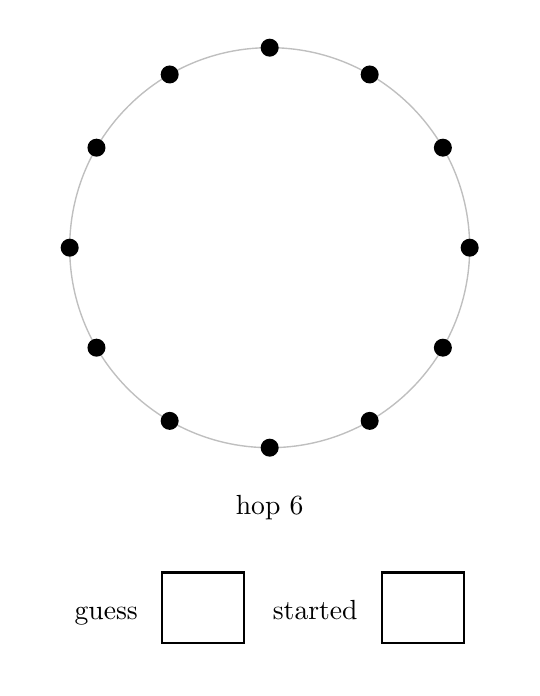
\begin{tikzpicture}[x=1in,y=1in]
\useasboundingbox (-1.21,-2.1) rectangle (1.21,1.1);
\draw[black!25, line width=0.5pt] (0,0) circle (1);
\fill[black] (0,1) circle (0.045);
\fill[black] (0.5,0.866) circle (0.045);
\fill[black] (0.866,0.5) circle (0.045);
\fill[black] (1,0) circle (0.045);
\fill[black] (0.866,-0.5) circle (0.045);
\fill[black] (0.5,-0.866) circle (0.045);
\fill[black] (0,-1) circle (0.045);
\fill[black] (-0.5,-0.866) circle (0.045);
\fill[black] (-0.866,-0.5) circle (0.045);
\fill[black] (-1,0) circle (0.045);
\fill[black] (-0.866,0.5) circle (0.045);
\fill[black] (-0.5,0.866) circle (0.045);
\node[font=\normalsize] at (0,-1.3) {hop 6};
\node[font=\normalsize] at (0,-1.8) {guess~\bx\quad started~\bx};
\end{tikzpicture}\hfill}\par
\vfill

\newpage
\par\vspace{0in}\noindent \prob{4} Cut out the two wheels on the last two pages and join them through the middle dots with a brass fastener. Setting the wheel to D means turning it until the inner A is next to the outer D. Each letter of a message on the inner wheel goes into code as the outer letter next to it, so with the wheel set to D, CAT goes into code as FDW. Set your wheel to D and find what each of these codes came from.\par
\par\vspace{0.25in}\noindent\begin{tikzpicture}[x=1in,y=1in]
\useasboundingbox (0,-0.5) rectangle (7.3,0.28);
\node[font=\Large\ttfamily, anchor=base] at (0.16,0) {V};
\draw[black!70, line width=0.7pt] (0.05,-0.44) -- (0.27,-0.44);
\node[font=\Large\ttfamily, anchor=base] at (0.48,0) {W};
\draw[black!70, line width=0.7pt] (0.37,-0.44) -- (0.59,-0.44);
\node[font=\Large\ttfamily, anchor=base] at (0.8,0) {D};
\draw[black!70, line width=0.7pt] (0.69,-0.44) -- (0.91,-0.44);
\node[font=\Large\ttfamily, anchor=base] at (1.12,0) {U};
\draw[black!70, line width=0.7pt] (1.01,-0.44) -- (1.23,-0.44);
\end{tikzpicture}\par
\par\vspace{0.2in}\noindent\begin{tikzpicture}[x=1in,y=1in]
\useasboundingbox (0,-0.5) rectangle (7.3,0.28);
\node[font=\Large\ttfamily, anchor=base] at (0.16,0) {I};
\draw[black!70, line width=0.7pt] (0.05,-0.44) -- (0.27,-0.44);
\node[font=\Large\ttfamily, anchor=base] at (0.48,0) {R};
\draw[black!70, line width=0.7pt] (0.37,-0.44) -- (0.59,-0.44);
\node[font=\Large\ttfamily, anchor=base] at (0.8,0) {A};
\draw[black!70, line width=0.7pt] (0.69,-0.44) -- (0.91,-0.44);
\end{tikzpicture}\par
\par\vspace{0.2in}\noindent\begin{tikzpicture}[x=1in,y=1in]
\useasboundingbox (0,-0.5) rectangle (7.3,0.28);
\node[font=\Large\ttfamily, anchor=base] at (0.16,0) {Z};
\draw[black!70, line width=0.7pt] (0.05,-0.44) -- (0.27,-0.44);
\node[font=\Large\ttfamily, anchor=base] at (0.48,0) {K};
\draw[black!70, line width=0.7pt] (0.37,-0.44) -- (0.59,-0.44);
\node[font=\Large\ttfamily, anchor=base] at (0.8,0) {H};
\draw[black!70, line width=0.7pt] (0.69,-0.44) -- (0.91,-0.44);
\node[font=\Large\ttfamily, anchor=base] at (1.12,0) {H};
\draw[black!70, line width=0.7pt] (1.01,-0.44) -- (1.23,-0.44);
\node[font=\Large\ttfamily, anchor=base] at (1.44,0) {O};
\draw[black!70, line width=0.7pt] (1.33,-0.44) -- (1.55,-0.44);
\end{tikzpicture}\par
\par\vspace{0.2in}\noindent\begin{tikzpicture}[x=1in,y=1in]
\useasboundingbox (0,-0.5) rectangle (7.3,0.28);
\node[font=\Large\ttfamily, anchor=base] at (0.16,0) {S};
\draw[black!70, line width=0.7pt] (0.05,-0.44) -- (0.27,-0.44);
\node[font=\Large\ttfamily, anchor=base] at (0.48,0) {H};
\draw[black!70, line width=0.7pt] (0.37,-0.44) -- (0.59,-0.44);
\node[font=\Large\ttfamily, anchor=base] at (0.8,0) {Q};
\draw[black!70, line width=0.7pt] (0.69,-0.44) -- (0.91,-0.44);
\node[font=\Large\ttfamily, anchor=base] at (1.12,0) {F};
\draw[black!70, line width=0.7pt] (1.01,-0.44) -- (1.23,-0.44);
\node[font=\Large\ttfamily, anchor=base] at (1.44,0) {L};
\draw[black!70, line width=0.7pt] (1.33,-0.44) -- (1.55,-0.44);
\node[font=\Large\ttfamily, anchor=base] at (1.76,0) {O};
\draw[black!70, line width=0.7pt] (1.65,-0.44) -- (1.87,-0.44);
\end{tikzpicture}\par
\par\vspace{0.2in}\noindent\begin{tikzpicture}[x=1in,y=1in]
\useasboundingbox (0,-0.5) rectangle (7.3,0.28);
\node[font=\Large\ttfamily, anchor=base] at (0.16,0) {L};
\draw[black!70, line width=0.7pt] (0.05,-0.44) -- (0.27,-0.44);
\node[font=\Large\ttfamily, anchor=base] at (0.8,0) {F};
\draw[black!70, line width=0.7pt] (0.69,-0.44) -- (0.91,-0.44);
\node[font=\Large\ttfamily, anchor=base] at (1.12,0) {D};
\draw[black!70, line width=0.7pt] (1.01,-0.44) -- (1.23,-0.44);
\node[font=\Large\ttfamily, anchor=base] at (1.44,0) {Q};
\draw[black!70, line width=0.7pt] (1.33,-0.44) -- (1.55,-0.44);
\node[font=\Large\ttfamily, anchor=base] at (2.08,0) {G};
\draw[black!70, line width=0.7pt] (1.97,-0.44) -- (2.19,-0.44);
\node[font=\Large\ttfamily, anchor=base] at (2.4,0) {U};
\draw[black!70, line width=0.7pt] (2.29,-0.44) -- (2.51,-0.44);
\node[font=\Large\ttfamily, anchor=base] at (2.72,0) {D};
\draw[black!70, line width=0.7pt] (2.61,-0.44) -- (2.83,-0.44);
\node[font=\Large\ttfamily, anchor=base] at (3.04,0) {Z};
\draw[black!70, line width=0.7pt] (2.93,-0.44) -- (3.15,-0.44);
\node[font=\Large\ttfamily, anchor=base] at (3.68,0) {D};
\draw[black!70, line width=0.7pt] (3.57,-0.44) -- (3.79,-0.44);
\node[font=\Large\ttfamily, anchor=base] at (4.32,0) {V};
\draw[black!70, line width=0.7pt] (4.21,-0.44) -- (4.43,-0.44);
\node[font=\Large\ttfamily, anchor=base] at (4.64,0) {W};
\draw[black!70, line width=0.7pt] (4.53,-0.44) -- (4.75,-0.44);
\node[font=\Large\ttfamily, anchor=base] at (4.96,0) {D};
\draw[black!70, line width=0.7pt] (4.85,-0.44) -- (5.07,-0.44);
\node[font=\Large\ttfamily, anchor=base] at (5.28,0) {U};
\draw[black!70, line width=0.7pt] (5.17,-0.44) -- (5.39,-0.44);
\end{tikzpicture}\par
\par\vspace{0.4in}\noindent \prob{5} Write a message of at least five words for your partner, and put it into code with a setting you choose. Swap codes and settings with your partner, and find your partner's message.\par
\par\vspace{0.05in}\noindent\begin{tikzpicture}[x=1in,y=1in]
\useasboundingbox (0,-2.05) rectangle (7.3,0);
\draw[black!55, line width=0.5pt] (0,-0.4) -- (7.3,-0.4);
\draw[black!55, line width=0.5pt] (0,-0.8) -- (7.3,-0.8);
\draw[black!55, line width=0.5pt] (0,-1.2) -- (7.3,-1.2);
\draw[black!55, line width=0.5pt] (0,-1.6) -- (7.3,-1.6);
\draw[black!55, line width=0.5pt] (0,-2) -- (7.3,-2);
\end{tikzpicture}\par
\vfill

\newpage
\par\vspace{0in}\noindent \prob{6} Before you draw each of these, guess how many times you will start and write your guess. Then draw it and write how many times you did start.\par
\par\vspace{0.3in}\noindent\makebox[\textwidth][s]{\hfill \begin{tikzpicture}[x=1in,y=1in]
\useasboundingbox (-1.8,-2.35) rectangle (1.8,1.35);
\draw[black!25, line width=0.5pt] (0,0) circle (1.25);
\fill[black] (0,1.25) circle (0.045);
\fill[black] (0.8035,0.9576) circle (0.045);
\fill[black] (1.231,0.2171) circle (0.045);
\fill[black] (1.0825,-0.625) circle (0.045);
\fill[black] (0.4275,-1.1746) circle (0.045);
\fill[black] (-0.4275,-1.1746) circle (0.045);
\fill[black] (-1.0825,-0.625) circle (0.045);
\fill[black] (-1.231,0.2171) circle (0.045);
\fill[black] (-0.8035,0.9576) circle (0.045);
\node[font=\normalsize] at (0,-1.55) {9 dots, hop 2};
\node[font=\normalsize] at (0,-2.05) {guess~\bx\quad started~\bx};
\end{tikzpicture}\hfill \begin{tikzpicture}[x=1in,y=1in]
\useasboundingbox (-1.8,-2.35) rectangle (1.8,1.35);
\draw[black!25, line width=0.5pt] (0,0) circle (1.25);
\fill[black] (0,1.25) circle (0.04);
\fill[black] (0.5084,1.1419) circle (0.04);
\fill[black] (0.9289,0.8364) circle (0.04);
\fill[black] (1.1888,0.3863) circle (0.04);
\fill[black] (1.2432,-0.1307) circle (0.04);
\fill[black] (1.0825,-0.625) circle (0.04);
\fill[black] (0.7347,-1.0113) circle (0.04);
\fill[black] (0.2599,-1.2227) circle (0.04);
\fill[black] (-0.2599,-1.2227) circle (0.04);
\fill[black] (-0.7347,-1.0113) circle (0.04);
\fill[black] (-1.0825,-0.625) circle (0.04);
\fill[black] (-1.2432,-0.1307) circle (0.04);
\fill[black] (-1.1888,0.3863) circle (0.04);
\fill[black] (-0.9289,0.8364) circle (0.04);
\fill[black] (-0.5084,1.1419) circle (0.04);
\node[font=\normalsize] at (0,-1.55) {15 dots, hop 5};
\node[font=\normalsize] at (0,-2.05) {guess~\bx\quad started~\bx};
\end{tikzpicture}\hfill}\par
\par\vspace{0.45in}\noindent\makebox[\textwidth][s]{\hfill \begin{tikzpicture}[x=1in,y=1in]
\useasboundingbox (-1.8,-2.35) rectangle (1.8,1.35);
\draw[black!25, line width=0.5pt] (0,0) circle (1.25);
\fill[black] (0,1.25) circle (0.04);
\fill[black] (0.4784,1.1548) circle (0.04);
\fill[black] (0.8839,0.8839) circle (0.04);
\fill[black] (1.1548,0.4784) circle (0.04);
\fill[black] (1.25,0) circle (0.04);
\fill[black] (1.1548,-0.4784) circle (0.04);
\fill[black] (0.8839,-0.8839) circle (0.04);
\fill[black] (0.4784,-1.1548) circle (0.04);
\fill[black] (0,-1.25) circle (0.04);
\fill[black] (-0.4784,-1.1548) circle (0.04);
\fill[black] (-0.8839,-0.8839) circle (0.04);
\fill[black] (-1.1548,-0.4784) circle (0.04);
\fill[black] (-1.25,0) circle (0.04);
\fill[black] (-1.1548,0.4784) circle (0.04);
\fill[black] (-0.8839,0.8839) circle (0.04);
\fill[black] (-0.4784,1.1548) circle (0.04);
\node[font=\normalsize] at (0,-1.55) {16 dots, hop 6};
\node[font=\normalsize] at (0,-2.05) {guess~\bx\quad started~\bx};
\end{tikzpicture}\hfill \begin{tikzpicture}[x=1in,y=1in]
\useasboundingbox (-1.8,-2.35) rectangle (1.8,1.35);
\draw[black!25, line width=0.5pt] (0,0) circle (1.25);
\fill[black] (0,1.25) circle (0.045);
\fill[black] (0.625,1.0825) circle (0.045);
\fill[black] (1.0825,0.625) circle (0.045);
\fill[black] (1.25,0) circle (0.045);
\fill[black] (1.0825,-0.625) circle (0.045);
\fill[black] (0.625,-1.0825) circle (0.045);
\fill[black] (0,-1.25) circle (0.045);
\fill[black] (-0.625,-1.0825) circle (0.045);
\fill[black] (-1.0825,-0.625) circle (0.045);
\fill[black] (-1.25,0) circle (0.045);
\fill[black] (-1.0825,0.625) circle (0.045);
\fill[black] (-0.625,1.0825) circle (0.045);
\node[font=\normalsize] at (0,-1.55) {12 dots, hop 8};
\node[font=\normalsize] at (0,-2.05) {guess~\bx\quad started~\bx};
\end{tikzpicture}\hfill}\par
\vfill

\newpage
\par\vspace{0in}\noindent \prob{7} On each of these rings, find a hop bigger than 3 that makes you start exactly 3 times, and draw it. If a ring has no such hop, explain why.\par
\par\vspace{0.25in}\noindent\makebox[\textwidth][s]{\hfill \begin{tikzpicture}[x=1in,y=1in]
\useasboundingbox (-1.8,-1.8) rectangle (1.8,1.3);
\draw[black!25, line width=0.5pt] (0,0) circle (1.2);
\fill[black] (0,1.2) circle (0.045);
\fill[black] (0.7713,0.9193) circle (0.045);
\fill[black] (1.1818,0.2084) circle (0.045);
\fill[black] (1.0392,-0.6) circle (0.045);
\fill[black] (0.4104,-1.1276) circle (0.045);
\fill[black] (-0.4104,-1.1276) circle (0.045);
\fill[black] (-1.0392,-0.6) circle (0.045);
\fill[black] (-1.1818,0.2084) circle (0.045);
\fill[black] (-0.7713,0.9193) circle (0.045);
\node[font=\normalsize] at (0,-1.5) {9 dots, hop \blank};
\end{tikzpicture}\hfill \begin{tikzpicture}[x=1in,y=1in]
\useasboundingbox (-1.8,-1.8) rectangle (1.8,1.3);
\draw[black!25, line width=0.5pt] (0,0) circle (1.2);
\fill[black] (0,1.2) circle (0.04);
\fill[black] (0.4592,1.1087) circle (0.04);
\fill[black] (0.8485,0.8485) circle (0.04);
\fill[black] (1.1087,0.4592) circle (0.04);
\fill[black] (1.2,0) circle (0.04);
\fill[black] (1.1087,-0.4592) circle (0.04);
\fill[black] (0.8485,-0.8485) circle (0.04);
\fill[black] (0.4592,-1.1087) circle (0.04);
\fill[black] (0,-1.2) circle (0.04);
\fill[black] (-0.4592,-1.1087) circle (0.04);
\fill[black] (-0.8485,-0.8485) circle (0.04);
\fill[black] (-1.1087,-0.4592) circle (0.04);
\fill[black] (-1.2,0) circle (0.04);
\fill[black] (-1.1087,0.4592) circle (0.04);
\fill[black] (-0.8485,0.8485) circle (0.04);
\fill[black] (-0.4592,1.1087) circle (0.04);
\node[font=\normalsize] at (0,-1.5) {16 dots, hop \blank};
\end{tikzpicture}\hfill}\par
\par\vspace{0.35in}\noindent\makebox[\textwidth][s]{\hfill \begin{tikzpicture}[x=1in,y=1in]
\useasboundingbox (-1.8,-1.8) rectangle (1.8,1.3);
\draw[black!25, line width=0.5pt] (0,0) circle (1.2);
\fill[black] (0,1.2) circle (0.04);
\fill[black] (0.4104,1.1276) circle (0.04);
\fill[black] (0.7713,0.9193) circle (0.04);
\fill[black] (1.0392,0.6) circle (0.04);
\fill[black] (1.1818,0.2084) circle (0.04);
\fill[black] (1.1818,-0.2084) circle (0.04);
\fill[black] (1.0392,-0.6) circle (0.04);
\fill[black] (0.7713,-0.9193) circle (0.04);
\fill[black] (0.4104,-1.1276) circle (0.04);
\fill[black] (0,-1.2) circle (0.04);
\fill[black] (-0.4104,-1.1276) circle (0.04);
\fill[black] (-0.7713,-0.9193) circle (0.04);
\fill[black] (-1.0392,-0.6) circle (0.04);
\fill[black] (-1.1818,-0.2084) circle (0.04);
\fill[black] (-1.1818,0.2084) circle (0.04);
\fill[black] (-1.0392,0.6) circle (0.04);
\fill[black] (-0.7713,0.9193) circle (0.04);
\fill[black] (-0.4104,1.1276) circle (0.04);
\node[font=\normalsize] at (0,-1.5) {18 dots, hop \blank};
\end{tikzpicture}\hfill \begin{tikzpicture}[x=1in,y=1in]
\useasboundingbox (-1.8,-1.8) rectangle (1.8,1.3);
\draw[black!25, line width=0.5pt] (0,0) circle (1.2);
\fill[black] (0,1.2) circle (0.04);
\fill[black] (0.4881,1.0963) circle (0.04);
\fill[black] (0.8918,0.803) circle (0.04);
\fill[black] (1.1413,0.3708) circle (0.04);
\fill[black] (1.1934,-0.1254) circle (0.04);
\fill[black] (1.0392,-0.6) circle (0.04);
\fill[black] (0.7053,-0.9708) circle (0.04);
\fill[black] (0.2495,-1.1738) circle (0.04);
\fill[black] (-0.2495,-1.1738) circle (0.04);
\fill[black] (-0.7053,-0.9708) circle (0.04);
\fill[black] (-1.0392,-0.6) circle (0.04);
\fill[black] (-1.1934,-0.1254) circle (0.04);
\fill[black] (-1.1413,0.3708) circle (0.04);
\fill[black] (-0.8918,0.803) circle (0.04);
\fill[black] (-0.4881,1.0963) circle (0.04);
\node[font=\normalsize] at (0,-1.5) {15 dots, hop \blank};
\end{tikzpicture}\hfill}\par
\par\vspace{0.1in}\noindent\begin{tikzpicture}[x=1in,y=1in]
\useasboundingbox (0,-1.25) rectangle (7.3,0);
\draw[black!55, line width=0.5pt] (0,-0.4) -- (7.3,-0.4);
\draw[black!55, line width=0.5pt] (0,-0.8) -- (7.3,-0.8);
\draw[black!55, line width=0.5pt] (0,-1.2) -- (7.3,-1.2);
\end{tikzpicture}\par
\vfill

\newpage
\par\vspace{0in}\noindent \prob{8} These messages were put into code with settings nobody wrote down. Find the messages.\par
\par\vspace{0.3in}\noindent\begin{tikzpicture}[x=1in,y=1in]
\useasboundingbox (0,-0.5) rectangle (7.3,0.28);
\node[font=\Large\ttfamily, anchor=base] at (0.16,0) {H};
\draw[black!70, line width=0.7pt] (0.05,-0.44) -- (0.27,-0.44);
\node[font=\Large\ttfamily, anchor=base] at (0.8,0) {Z};
\draw[black!70, line width=0.7pt] (0.69,-0.44) -- (0.91,-0.44);
\node[font=\Large\ttfamily, anchor=base] at (1.12,0) {A};
\draw[black!70, line width=0.7pt] (1.01,-0.44) -- (1.23,-0.44);
\node[font=\Large\ttfamily, anchor=base] at (1.44,0) {H};
\draw[black!70, line width=0.7pt] (1.33,-0.44) -- (1.55,-0.44);
\node[font=\Large\ttfamily, anchor=base] at (1.76,0) {Y};
\draw[black!70, line width=0.7pt] (1.65,-0.44) -- (1.87,-0.44);
\node[font=\Large\ttfamily, anchor=base] at (2.4,0) {J};
\draw[black!70, line width=0.7pt] (2.29,-0.44) -- (2.51,-0.44);
\node[font=\Large\ttfamily, anchor=base] at (2.72,0) {H};
\draw[black!70, line width=0.7pt] (2.61,-0.44) -- (2.83,-0.44);
\node[font=\Large\ttfamily, anchor=base] at (3.04,0) {U};
\draw[black!70, line width=0.7pt] (2.93,-0.44) -- (3.15,-0.44);
\node[font=\Large\ttfamily, anchor=base] at (3.68,0) {O};
\draw[black!70, line width=0.7pt] (3.57,-0.44) -- (3.79,-0.44);
\node[font=\Large\ttfamily, anchor=base] at (4,0) {H};
\draw[black!70, line width=0.7pt] (3.89,-0.44) -- (4.11,-0.44);
\node[font=\Large\ttfamily, anchor=base] at (4.32,0) {C};
\draw[black!70, line width=0.7pt] (4.21,-0.44) -- (4.43,-0.44);
\node[font=\Large\ttfamily, anchor=base] at (4.64,0) {L};
\draw[black!70, line width=0.7pt] (4.53,-0.44) -- (4.75,-0.44);
\node[font=\Large\ttfamily, anchor=base] at (5.28,0) {A};
\draw[black!70, line width=0.7pt] (5.17,-0.44) -- (5.39,-0.44);
\node[font=\Large\ttfamily, anchor=base] at (5.6,0) {L};
\draw[black!70, line width=0.7pt] (5.49,-0.44) -- (5.71,-0.44);
\node[font=\Large\ttfamily, anchor=base] at (5.92,0) {U};
\draw[black!70, line width=0.7pt] (5.81,-0.44) -- (6.03,-0.44);
\end{tikzpicture}\par
\par\vspace{0.12in}\noindent\begin{tikzpicture}[x=1in,y=1in]
\useasboundingbox (0,-0.5) rectangle (7.3,0.28);
\node[font=\Large\ttfamily, anchor=base] at (0.16,0) {W};
\draw[black!70, line width=0.7pt] (0.05,-0.44) -- (0.27,-0.44);
\node[font=\Large\ttfamily, anchor=base] at (0.48,0) {V};
\draw[black!70, line width=0.7pt] (0.37,-0.44) -- (0.59,-0.44);
\node[font=\Large\ttfamily, anchor=base] at (0.8,0) {P};
\draw[black!70, line width=0.7pt] (0.69,-0.44) -- (0.91,-0.44);
\node[font=\Large\ttfamily, anchor=base] at (1.12,0) {U};
\draw[black!70, line width=0.7pt] (1.01,-0.44) -- (1.23,-0.44);
\node[font=\Large\ttfamily, anchor=base] at (1.44,0) {A};
\draw[black!70, line width=0.7pt] (1.33,-0.44) -- (1.55,-0.44);
\node[font=\Large\ttfamily, anchor=base] at (1.76,0) {Z};
\draw[black!70, line width=0.7pt] (1.65,-0.44) -- (1.87,-0.44);
\end{tikzpicture}\par
\par\vspace{0.35in}\noindent\begin{tikzpicture}[x=1in,y=1in]
\useasboundingbox (0,-0.5) rectangle (7.3,0.28);
\node[font=\Large\ttfamily, anchor=base] at (0.16,0) {C};
\draw[black!70, line width=0.7pt] (0.05,-0.44) -- (0.27,-0.44);
\node[font=\Large\ttfamily, anchor=base] at (0.48,0) {U};
\draw[black!70, line width=0.7pt] (0.37,-0.44) -- (0.59,-0.44);
\node[font=\Large\ttfamily, anchor=base] at (0.8,0) {U};
\draw[black!70, line width=0.7pt] (0.69,-0.44) -- (0.91,-0.44);
\node[font=\Large\ttfamily, anchor=base] at (1.12,0) {J};
\draw[black!70, line width=0.7pt] (1.01,-0.44) -- (1.23,-0.44);
\node[font=\Large\ttfamily, anchor=base] at (1.76,0) {C};
\draw[black!70, line width=0.7pt] (1.65,-0.44) -- (1.87,-0.44);
\node[font=\Large\ttfamily, anchor=base] at (2.08,0) {U};
\draw[black!70, line width=0.7pt] (1.97,-0.44) -- (2.19,-0.44);
\node[font=\Large\ttfamily, anchor=base] at (2.72,0) {R};
\draw[black!70, line width=0.7pt] (2.61,-0.44) -- (2.83,-0.44);
\node[font=\Large\ttfamily, anchor=base] at (3.04,0) {O};
\draw[black!70, line width=0.7pt] (2.93,-0.44) -- (3.15,-0.44);
\node[font=\Large\ttfamily, anchor=base] at (3.68,0) {J};
\draw[black!70, line width=0.7pt] (3.57,-0.44) -- (3.79,-0.44);
\node[font=\Large\ttfamily, anchor=base] at (4,0) {X};
\draw[black!70, line width=0.7pt] (3.89,-0.44) -- (4.11,-0.44);
\node[font=\Large\ttfamily, anchor=base] at (4.32,0) {U};
\draw[black!70, line width=0.7pt] (4.21,-0.44) -- (4.43,-0.44);
\node[font=\Large\ttfamily, anchor=base] at (4.96,0) {R};
\draw[black!70, line width=0.7pt] (4.85,-0.44) -- (5.07,-0.44);
\node[font=\Large\ttfamily, anchor=base] at (5.28,0) {Y};
\draw[black!70, line width=0.7pt] (5.17,-0.44) -- (5.39,-0.44);
\node[font=\Large\ttfamily, anchor=base] at (5.6,0) {W};
\draw[black!70, line width=0.7pt] (5.49,-0.44) -- (5.71,-0.44);
\end{tikzpicture}\par
\par\vspace{0.12in}\noindent\begin{tikzpicture}[x=1in,y=1in]
\useasboundingbox (0,-0.5) rectangle (7.3,0.28);
\node[font=\Large\ttfamily, anchor=base] at (0.16,0) {J};
\draw[black!70, line width=0.7pt] (0.05,-0.44) -- (0.27,-0.44);
\node[font=\Large\ttfamily, anchor=base] at (0.48,0) {H};
\draw[black!70, line width=0.7pt] (0.37,-0.44) -- (0.59,-0.44);
\node[font=\Large\ttfamily, anchor=base] at (0.8,0) {U};
\draw[black!70, line width=0.7pt] (0.69,-0.44) -- (0.91,-0.44);
\node[font=\Large\ttfamily, anchor=base] at (1.12,0) {U};
\draw[black!70, line width=0.7pt] (1.01,-0.44) -- (1.23,-0.44);
\end{tikzpicture}\par
\par\vspace{0.6in}\noindent \prob{9} Sam put a word into code. Then he put that code into code again with a second setting, and he got his word back. Find the second setting for each of these first settings.\par
\par\vspace{0.3in}\noindent\makebox[\textwidth][c]{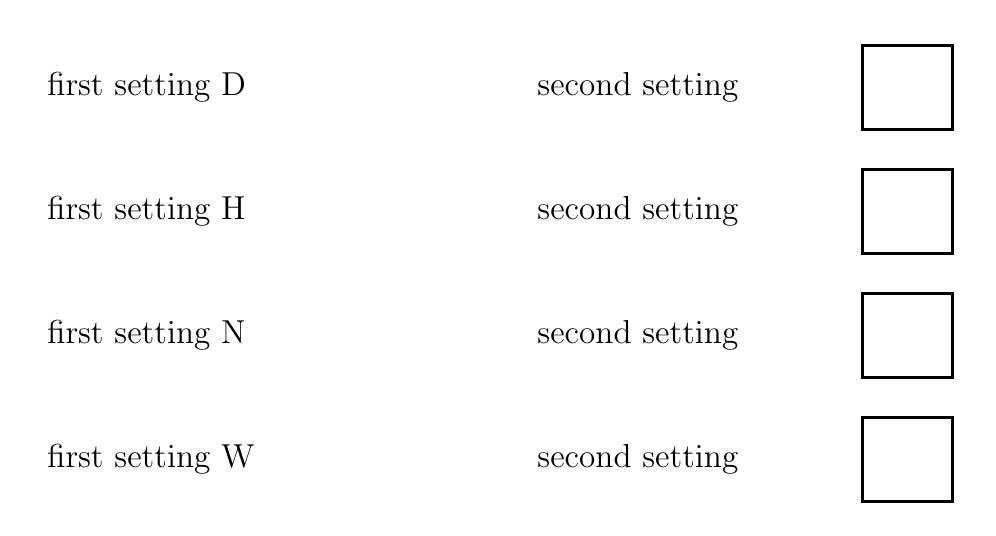
\begin{tikzpicture}[x=1in,y=1in]
\useasboundingbox (-0.05,-2.1) rectangle (4.65,0.3);
\node[font=\large, anchor=west] at (0,0) {first setting D};
\node[font=\large, anchor=west] at (2.45,0) {second setting};
\draw[line width=1pt] (4.125,-0.21) rectangle (4.575,0.21);
\node[font=\large, anchor=west] at (0,-0.62) {first setting H};
\node[font=\large, anchor=west] at (2.45,-0.62) {second setting};
\draw[line width=1pt] (4.125,-0.83) rectangle (4.575,-0.41);
\node[font=\large, anchor=west] at (0,-1.24) {first setting N};
\node[font=\large, anchor=west] at (2.45,-1.24) {second setting};
\draw[line width=1pt] (4.125,-1.45) rectangle (4.575,-1.03);
\node[font=\large, anchor=west] at (0,-1.86) {first setting W};
\node[font=\large, anchor=west] at (2.45,-1.86) {second setting};
\draw[line width=1pt] (4.125,-2.07) rectangle (4.575,-1.65);
\end{tikzpicture}}\par
\vfill

\newpage
\par\vspace{0in}\noindent\makebox[\textwidth][c]{\begin{tikzpicture}[x=1in,y=1in]
\useasboundingbox (0,0) rectangle (7.3,8.9);
\draw[line width=1.4pt] (3.65,4.45) circle (2.75);
\node[font=\bfseries\LARGE, rotate=0] at (3.65,6.88) {\underline{A}};
\draw[line width=0.6pt] (3.9007,6.5148) -- (3.9815,7.1799);
\node[font=\bfseries\LARGE, rotate=-13.8462] at (4.2315,6.8094) {\underline{B}};
\draw[line width=0.6pt] (4.3876,6.3948) -- (4.6252,7.0213);
\node[font=\bfseries\LARGE, rotate=-27.6923] at (4.7793,6.6017) {\underline{C}};
\draw[line width=0.6pt] (4.8316,6.1618) -- (5.2122,6.7132);
\node[font=\bfseries\LARGE, rotate=-41.5385] at (5.2614,6.2689) {\underline{D}};
\draw[line width=0.6pt] (5.2069,5.8293) -- (5.7084,6.2736);
\node[font=\bfseries\LARGE, rotate=-55.3846] at (5.6499,5.8304) {\underline{E}};
\draw[line width=0.6pt] (5.4917,5.4166) -- (6.085,5.728);
\node[font=\bfseries\LARGE, rotate=-69.2308] at (5.9221,5.3117) {\underline{F}};
\draw[line width=0.6pt] (5.6696,4.9478) -- (6.3201,5.1081);
\node[font=\bfseries\LARGE, rotate=-83.0769] at (6.0623,4.7429) {\underline{G}};
\draw[line width=0.6pt] (5.73,4.45) -- (6.4,4.45);
\node[font=\bfseries\LARGE, rotate=-96.9231] at (6.0623,4.1571) {\underline{H}};
\draw[line width=0.6pt] (5.6696,3.9522) -- (6.3201,3.7919);
\node[font=\bfseries\LARGE, rotate=-110.7692] at (5.9221,3.5883) {\underline{I}};
\draw[line width=0.6pt] (5.4917,3.4834) -- (6.085,3.172);
\node[font=\bfseries\LARGE, rotate=-124.6154] at (5.6499,3.0696) {\underline{J}};
\draw[line width=0.6pt] (5.2069,3.0707) -- (5.7084,2.6264);
\node[font=\bfseries\LARGE, rotate=-138.4615] at (5.2614,2.6311) {\underline{K}};
\draw[line width=0.6pt] (4.8316,2.7382) -- (5.2122,2.1868);
\node[font=\bfseries\LARGE, rotate=-152.3077] at (4.7793,2.2983) {\underline{L}};
\draw[line width=0.6pt] (4.3876,2.5052) -- (4.6252,1.8787);
\node[font=\bfseries\LARGE, rotate=-166.1538] at (4.2315,2.0906) {\underline{M}};
\draw[line width=0.6pt] (3.9007,2.3852) -- (3.9815,1.7201);
\node[font=\bfseries\LARGE, rotate=-180] at (3.65,2.02) {\underline{N}};
\draw[line width=0.6pt] (3.3993,2.3852) -- (3.3185,1.7201);
\node[font=\bfseries\LARGE, rotate=-193.8462] at (3.0685,2.0906) {\underline{O}};
\draw[line width=0.6pt] (2.9124,2.5052) -- (2.6748,1.8787);
\node[font=\bfseries\LARGE, rotate=-207.6923] at (2.5207,2.2983) {\underline{P}};
\draw[line width=0.6pt] (2.4684,2.7382) -- (2.0878,2.1868);
\node[font=\bfseries\LARGE, rotate=-221.5385] at (2.0386,2.6311) {\underline{Q}};
\draw[line width=0.6pt] (2.0931,3.0707) -- (1.5916,2.6264);
\node[font=\bfseries\LARGE, rotate=-235.3846] at (1.6501,3.0696) {\underline{R}};
\draw[line width=0.6pt] (1.8083,3.4834) -- (1.215,3.172);
\node[font=\bfseries\LARGE, rotate=-249.2308] at (1.3779,3.5883) {\underline{S}};
\draw[line width=0.6pt] (1.6304,3.9522) -- (0.9799,3.7919);
\node[font=\bfseries\LARGE, rotate=-263.0769] at (1.2377,4.1571) {\underline{T}};
\draw[line width=0.6pt] (1.57,4.45) -- (0.9,4.45);
\node[font=\bfseries\LARGE, rotate=-276.9231] at (1.2377,4.7429) {\underline{U}};
\draw[line width=0.6pt] (1.6304,4.9478) -- (0.9799,5.1081);
\node[font=\bfseries\LARGE, rotate=-290.7692] at (1.3779,5.3117) {\underline{V}};
\draw[line width=0.6pt] (1.8083,5.4166) -- (1.215,5.728);
\node[font=\bfseries\LARGE, rotate=-304.6154] at (1.6501,5.8304) {\underline{W}};
\draw[line width=0.6pt] (2.0931,5.8293) -- (1.5916,6.2736);
\node[font=\bfseries\LARGE, rotate=-318.4615] at (2.0386,6.2689) {\underline{X}};
\draw[line width=0.6pt] (2.4684,6.1618) -- (2.0878,6.7132);
\node[font=\bfseries\LARGE, rotate=-332.3077] at (2.5207,6.6017) {\underline{Y}};
\draw[line width=0.6pt] (2.9124,6.3948) -- (2.6748,7.0213);
\node[font=\bfseries\LARGE, rotate=-346.1538] at (3.0685,6.8094) {\underline{Z}};
\draw[line width=0.6pt] (3.3993,6.5148) -- (3.3185,7.1799);
\fill (3.65,4.45) circle (0.05);
\draw[line width=0.6pt] (3.47,4.45) -- (3.83,4.45) (3.65,4.27) -- (3.65,4.63);
\end{tikzpicture}}\par
\vfill

\newpage
\par\vspace{0in}\noindent\makebox[\textwidth][c]{\begin{tikzpicture}[x=1in,y=1in]
\useasboundingbox (0,0) rectangle (7.3,8.9);
\draw[line width=1.4pt] (3.65,4.45) circle (2);
\node[font=\bfseries\Large, rotate=0] at (3.65,6.15) {\underline{A}};
\draw[line width=0.6pt] (3.8212,5.8596) -- (3.8911,6.4354);
\node[font=\bfseries\Large, rotate=-13.8462] at (4.0568,6.1006) {\underline{B}};
\draw[line width=0.6pt] (4.1535,5.7777) -- (4.3592,6.32);
\node[font=\bfseries\Large, rotate=-27.6923] at (4.44,5.9553) {\underline{C}};
\draw[line width=0.6pt] (4.4567,5.6186) -- (4.7861,6.096);
\node[font=\bfseries\Large, rotate=-41.5385] at (4.7773,5.7225) {\underline{D}};
\draw[line width=0.6pt] (4.7129,5.3916) -- (5.147,5.7762);
\node[font=\bfseries\Large, rotate=-55.3846] at (5.0491,5.4157) {\underline{E}};
\draw[line width=0.6pt] (4.9073,5.1099) -- (5.4209,5.3794);
\node[font=\bfseries\Large, rotate=-69.2308] at (5.2395,5.0528) {\underline{F}};
\draw[line width=0.6pt] (5.0287,4.7898) -- (5.5919,4.9286);
\node[font=\bfseries\Large, rotate=-83.0769] at (5.3376,4.6549) {\underline{G}};
\draw[line width=0.6pt] (5.07,4.45) -- (5.65,4.45);
\node[font=\bfseries\Large, rotate=-96.9231] at (5.3376,4.2451) {\underline{H}};
\draw[line width=0.6pt] (5.0287,4.1102) -- (5.5919,3.9714);
\node[font=\bfseries\Large, rotate=-110.7692] at (5.2395,3.8472) {\underline{I}};
\draw[line width=0.6pt] (4.9073,3.7901) -- (5.4209,3.5206);
\node[font=\bfseries\Large, rotate=-124.6154] at (5.0491,3.4843) {\underline{J}};
\draw[line width=0.6pt] (4.7129,3.5084) -- (5.147,3.1238);
\node[font=\bfseries\Large, rotate=-138.4615] at (4.7773,3.1775) {\underline{K}};
\draw[line width=0.6pt] (4.4567,3.2814) -- (4.7861,2.804);
\node[font=\bfseries\Large, rotate=-152.3077] at (4.44,2.9447) {\underline{L}};
\draw[line width=0.6pt] (4.1535,3.1223) -- (4.3592,2.58);
\node[font=\bfseries\Large, rotate=-166.1538] at (4.0568,2.7994) {\underline{M}};
\draw[line width=0.6pt] (3.8212,3.0404) -- (3.8911,2.4646);
\node[font=\bfseries\Large, rotate=-180] at (3.65,2.75) {\underline{N}};
\draw[line width=0.6pt] (3.4788,3.0404) -- (3.4089,2.4646);
\node[font=\bfseries\Large, rotate=-193.8462] at (3.2432,2.7994) {\underline{O}};
\draw[line width=0.6pt] (3.1465,3.1223) -- (2.9408,2.58);
\node[font=\bfseries\Large, rotate=-207.6923] at (2.86,2.9447) {\underline{P}};
\draw[line width=0.6pt] (2.8433,3.2814) -- (2.5139,2.804);
\node[font=\bfseries\Large, rotate=-221.5385] at (2.5227,3.1775) {\underline{Q}};
\draw[line width=0.6pt] (2.5871,3.5084) -- (2.153,3.1238);
\node[font=\bfseries\Large, rotate=-235.3846] at (2.2509,3.4843) {\underline{R}};
\draw[line width=0.6pt] (2.3927,3.7901) -- (1.8791,3.5206);
\node[font=\bfseries\Large, rotate=-249.2308] at (2.0605,3.8472) {\underline{S}};
\draw[line width=0.6pt] (2.2713,4.1102) -- (1.7081,3.9714);
\node[font=\bfseries\Large, rotate=-263.0769] at (1.9624,4.2451) {\underline{T}};
\draw[line width=0.6pt] (2.23,4.45) -- (1.65,4.45);
\node[font=\bfseries\Large, rotate=-276.9231] at (1.9624,4.6549) {\underline{U}};
\draw[line width=0.6pt] (2.2713,4.7898) -- (1.7081,4.9286);
\node[font=\bfseries\Large, rotate=-290.7692] at (2.0605,5.0528) {\underline{V}};
\draw[line width=0.6pt] (2.3927,5.1099) -- (1.8791,5.3794);
\node[font=\bfseries\Large, rotate=-304.6154] at (2.2509,5.4157) {\underline{W}};
\draw[line width=0.6pt] (2.5871,5.3916) -- (2.153,5.7762);
\node[font=\bfseries\Large, rotate=-318.4615] at (2.5227,5.7225) {\underline{X}};
\draw[line width=0.6pt] (2.8433,5.6186) -- (2.5139,6.096);
\node[font=\bfseries\Large, rotate=-332.3077] at (2.86,5.9553) {\underline{Y}};
\draw[line width=0.6pt] (3.1465,5.7777) -- (2.9408,6.32);
\node[font=\bfseries\Large, rotate=-346.1538] at (3.2432,6.1006) {\underline{Z}};
\draw[line width=0.6pt] (3.4788,5.8596) -- (3.4089,6.4354);
\fill (3.65,4.45) circle (0.05);
\draw[line width=0.6pt] (3.47,4.45) -- (3.83,4.45) (3.65,4.27) -- (3.65,4.63);
\end{tikzpicture}}\par
\vfill

\end{document}
